\documentclass[a0paper,portrait]{baposter}

%----------------------------------------------------------------------------------------
%	SIMPLE BOXED ENVIRONMENT
%----------------------------------------------------------------------------------------

\usepackage{wrapfig}
\usepackage{lmodern}

\usepackage[utf8]{inputenc} %unicode support
\usepackage[T1]{fontenc}
\usepackage{amsmath}

\selectcolormodel{cmyk}

\graphicspath{{figures/}} % Directory in which figures are stored


\newcommand{\compresslist}{%
\setlength{\itemsep}{0pt}%
\setlength{\parskip}{1pt}%
\setlength{\parsep}{0pt}%
}

\newenvironment{boenumerate}
  {\begin{enumerate}\renewcommand\labelenumi{\textbf\theenumi.}}
  {\end{enumerate}}

% kaobox (while tcolorbox may be more rich, I find it too complicated so I prefer mdframed)
\RequirePackage{tikz}
\RequirePackage[framemethod=TikZ]{mdframed}

%\mdfsetup{skipabove=\topskip,skipbelow=0pt}
\mdfdefinestyle{kaoboxstyle}{
	skipabove=1.5\topskip,
	skipbelow=.5\topskip,
	rightmargin=0pt,
	leftmargin=0pt,
	%innertopmargin=3pt,
	%innerbottommargin=3pt,
	innerrightmargin=7pt,
	innerleftmargin=7pt,
	topline=false,
	bottomline=false,
	rightline=false,
	leftline=false,
	%linewidth=1pt,
	%roundcorner=0pt,
	%font={},
	%frametitlefont={},
	frametitlerule=true,
	linecolor=black,
	%backgroundcolor=LightBlue,
	fontcolor=black,
	%frametitlebackgroundcolor=LightBlue,
}

\newmdenv[
	style=kaoboxstyle,
	backgroundcolor=lightgreen!25,
	frametitlebackgroundcolor=lightgreen!25,
]{kaobox}


\begin{document}


\definecolor{darkgreen}{cmyk}{0.8,0,0.8,0.45}
\definecolor{lightgreen}{cmyk}{0.8,0,0.8,0.25}

\begin{poster}
{
grid=false,
headerborder=open, % Adds a border around the header of content boxes
colspacing=1em, % Column spacing
bgColorOne=white, % Background color for the gradient on the left side of the poster
bgColorTwo=white, % Background color for the gradient on the right side of the poster
borderColor=darkgreen, % Border color
headerColorOne=lightgreen, % Background color for the header in the content boxes (left side)
headerColorTwo=lightgreen, % Background color for the header in the content boxes (right side)
headerFontColor=white, % Text color for the header text in the content boxes
boxColorOne=white, % Background color of the content boxes
textborder=rounded, %rectangle, % Format of the border around content boxes, can be: none, bars, coils, triangles, rectangle, rounded, roundedsmall, roundedright or faded
eyecatcher=false, % Set to false for ignoring the left logo in the title and move the title left
headerheight=0.11\textheight, % Height of the header
headershape=rounded, % Specify the rounded corner in the content box headers, can be: rectangle, small-rounded, roundedright, roundedleft or rounded
headershade=plain,
headerfont=\Large\textsf, % Large, bold and sans serif font in the headers of content boxes
%textfont={\setlength{\parindent}{1.5em}}, % Uncomment for paragraph indentation
linewidth=2pt % Width of the border lines around content boxes
}
{}
%
%----------------------------------------------------------------------------------------
%	TITLE AND AUTHOR NAME
%----------------------------------------------------------------------------------------
%
{
\textsf %Sans Serif
{A Hydrogen Economy at Scale?
}
} % Poster title
% {\vspace{1em} Marta Stepniewska, Pawel Siedlecki\\ % Author names
% {\small \vspace{0.7em} Department of Bioinformatics, Institute of Biochemistry and Biophysics, PAS, Warsaw, Pawinskiego 5a}} % Author email addresses
{\sf\vspace{0.5em}\\
A look into the promises and challenges of hydrogen as an energy commodity.
}
{
\includegraphics[width=35mm,scale=0.35]{favpng_question-mark-logo-information}} % University/lab logo


\headerbox{1. Case Study}{name=introduction,column=0,row=0, span=3}{
The main energy storage option discussed in the media are the batteries. We have however seen that the most common form of energy storage in today's world was by far pumped hydroelectric storage. Another form of energy storage is gaining traction, hydrogen. In this section we will take a quick look at what its potential is.
}


\headerbox{2. Hydrogen Economy}{name=model,column=0,below=introduction,span=1}{

Hydrogen is a versatile element, which can be used to store energy, or to power engines. It can replace gas in vehicles, and help decarbonize some industrial sectors. However, it needs to be produced, stored, and distributed, in very energy intensive processes.

The three main issues of what has been referred to as hydrogen economy are thus:
\begin{itemize}
\item Production
\item Storage
\item Distribution
\end{itemize}

In this factsheet, we discuss the first order limitations to keep in mind.

}


\headerbox{3. Current market}{name=mcs,column=0,below=model,span=1}{

Hydrogen production already exists today. Its main uses are in the agricultural industry (fertilizers) and in the petroleum industry (refining). Approximately 75 MT of hydrogen is produced each year, and it is very important to keep in mind that 95\% of that production is not clean, and a carbon emitter. This stems from the economical use of natural gas or coal to produce hydrogen.

A process known as electrolysis allows, given a substantial amount of energy, to separate hydrogen from oxygen in water. If renewable sources of electricity are used, this is called "green hydrogen".


% Image attribution:
% https://rmi.org/the-truth-about-hydrogen/
%Source data from Balat, M. “Potential importance of hydrogen as a future solution to environmental and transportation problems,” International Journal of Hydrogen EnergyVolume 33, Issue 15, August 2008, Pages 4013-4029.
\begin{center}
    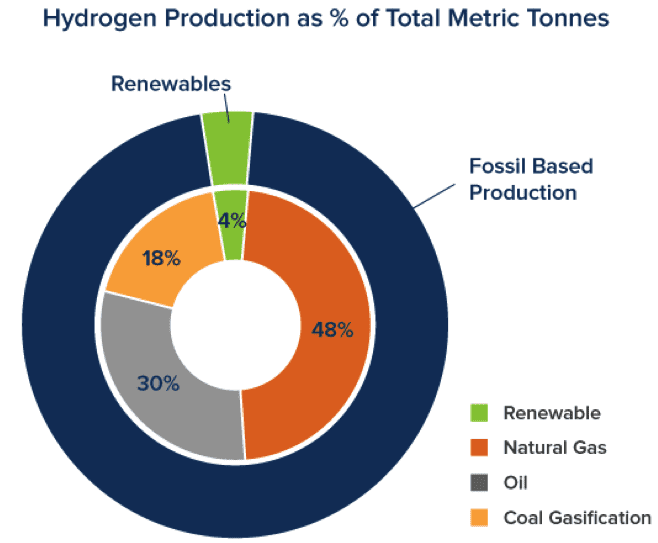
\includegraphics[width=\linewidth]{hydrogen_chart_smaller}
\end{center}

}

\headerbox{4. Computations}{name=screen,span=2,column=1,below=introduction}{ % To reduce this block to 1 column width, remove 'span=2'

%Image attribution:
%https://www.irena.org/energytransition/Power-Sector-Transformation/Hydrogen-from-Renewable-Power
\begin{center}
    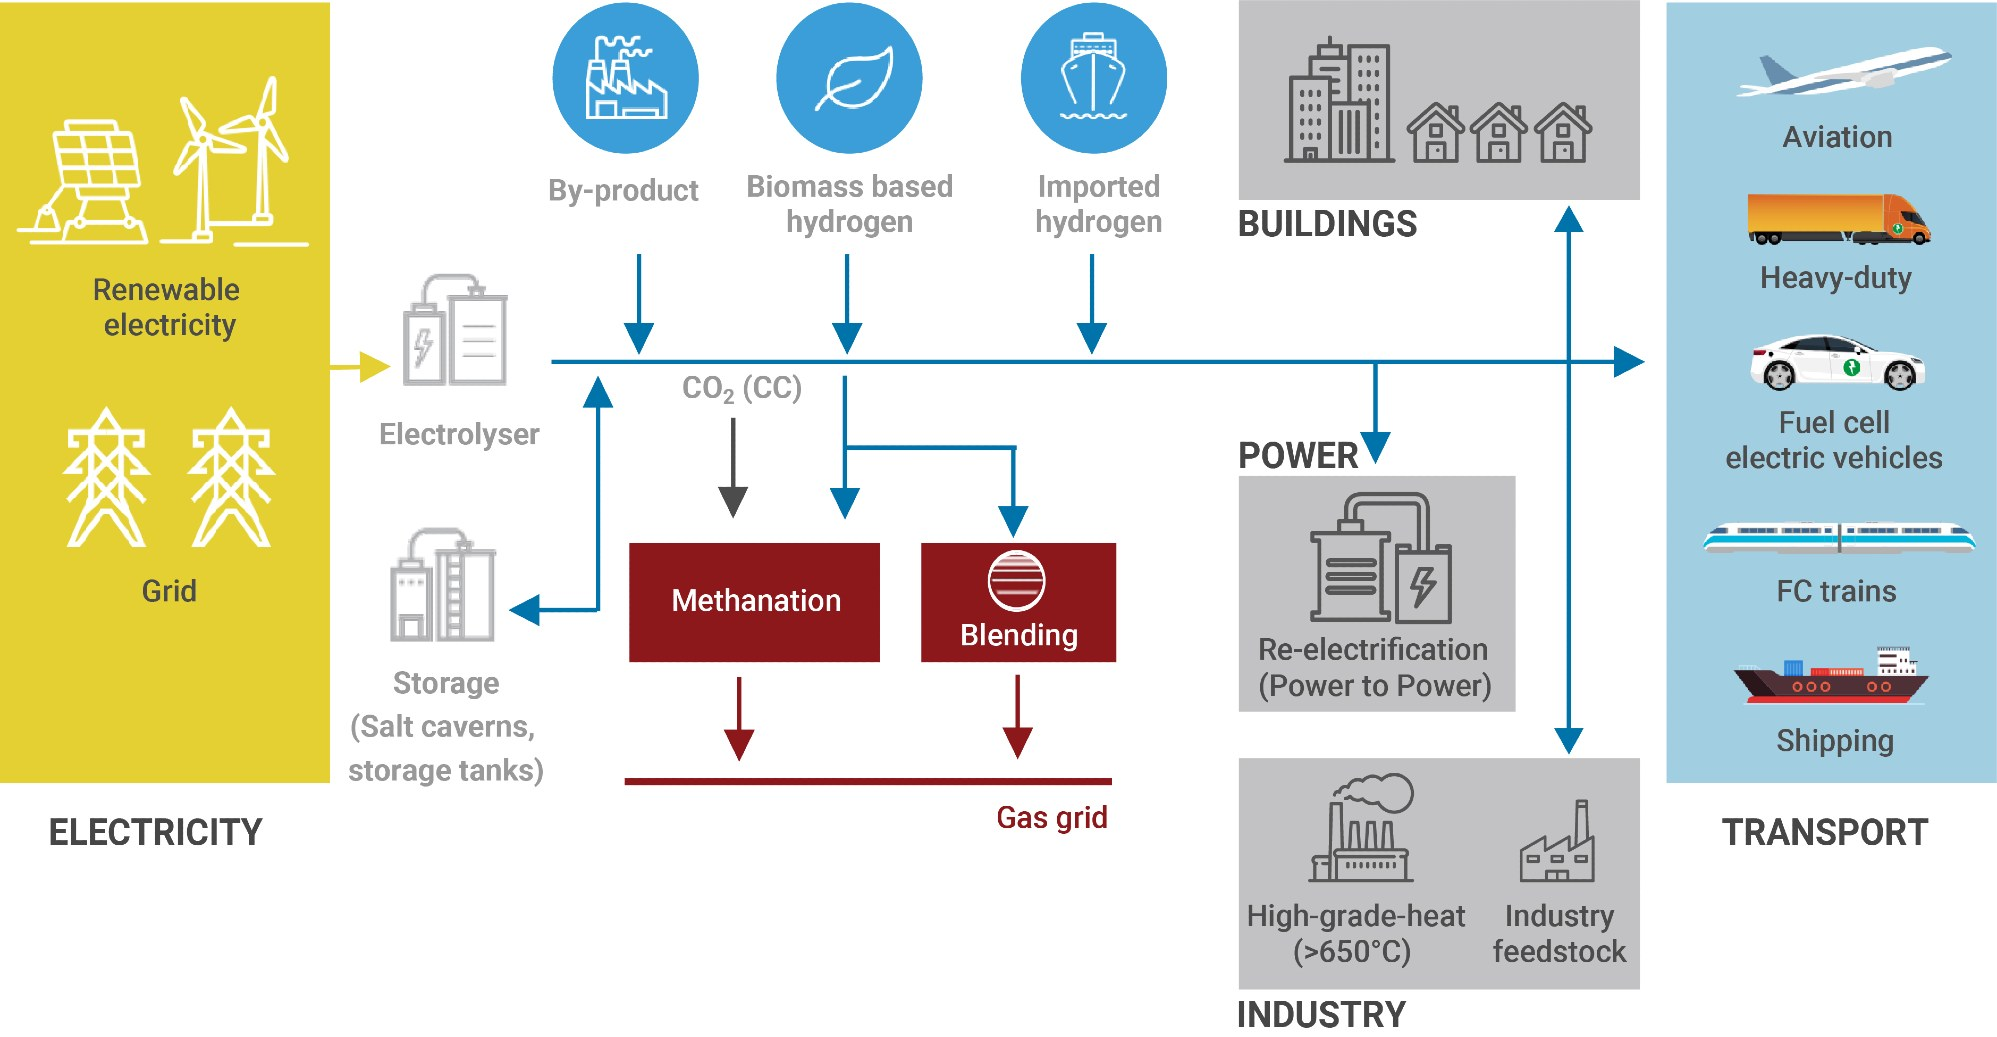
\includegraphics[width=\linewidth]{hydrogen_uses_irena}
\end{center}

We can see a quick schema representing a hydrogen economy. Excess generation from renewable sources would be used to power electrolyzers, which produce the hydrogen that is then distributed to various end-point, a carbon-free resource.

}

\headerbox{5. Limitations}{name=sea,span=2,column=1,below=screen}{ % To reduce this block to 1 column width, remove 'span=2'

Several important limitations are to keep in mind. First and foremost, the efficiency of the \textit{power-gas-power} cycle is very low. Electrolysis is roughly 75\% efficient. A fuel cell (hydrogen to power) is typically 50\% efficient. This means that the round-trip efficiency is less than 40\%. This is a very inefficient storage potential compared to batteries or pumped storage, and you need a much larger energy input. Speaking of energy, we produce today around 75 MT of hydrogen in the world, from non-electrolysis (and non-clean) processes. One need approximately 50 kWh of energy to produce 1 kilogram of hydrogen through electrolysis. Simply switching the existing production to green hydrogen production would demand around 3500 TWh per year. To give you a comparison point, the entire European Union generates under 3000 TWh, and the USA around 4000 TWh, of electricity every year. Water usage is also an important consideration. It takes 27 gallons of water to produce 1 kg of Hydrogen. Water becoming a rare commodity in a lot of places, this may pause a significant problem. On an engineering side, the challenges of developing an infrastructure able to store hydrogen are massive, and would require massive investments.


\begin{kaobox}[frametitle=Common Questions]
\begin{itemize}
\item \textit{What about using ocean water?}

This would change a lot of things from a water resource perspective. Seawater can corrode the electrolyzer, and needs to be purified. Desalination is an option, but at a large energy cost too. This would likely make the technology more expensive than it could afford to be.

\item \textit{So what if it's expensive?}

Even if you forget the impact on people, for transportation notably, remember that this technology competes with itself too. Electrolysis is one of the two main processes to produce hydrogen, the other one being "steam reforming", which uses natural gas, emits carbon, and is cheaper.

\end{itemize}
\end{kaobox}

}


\headerbox{6. Conclusions}{name=conclusion,column=1,below=sea,span=2,above=bottom}{
% DeCAF is a chemoinformatical tool that can be helpful in ligand-based drug design.
% It provides a comprehensive molecule description and a fast algorithms for comparing and aligning multiple ligands.
\begin{boenumerate}\compresslist
    \item Hydrogen has the potential to be useful in the future energy mix
    \item Its limitations, in terms of energy demands and water needs notably, suggest that it cannot sustain a large scale operation by itself
    \item A large hydrogen economy is unlikely to happen in reasonable amounts of time, given its infrastructure, external challenges, and competitors (batteries for electric vehicles for example).
\end{boenumerate}
}


\headerbox{7. Go further}{name=references,column=0,span=1,below=mcs,above=bottom}{


An interesting thing to keep in mind is that higher efficiency is obtained thanks to precious materials such as platinum. We would face the same finite materials problem we have discussed previously to maintain a high efficiency (and thus competitiveness).

Link to the Pumped Storage Case Study

Link to the Materials limitation Case Study

}

\end{poster}

\end{document}
